\chapter{Algorytm sterowania ruchem drogowym}
\section{Algorytm}
\begin{figure}[h]
    \centering
    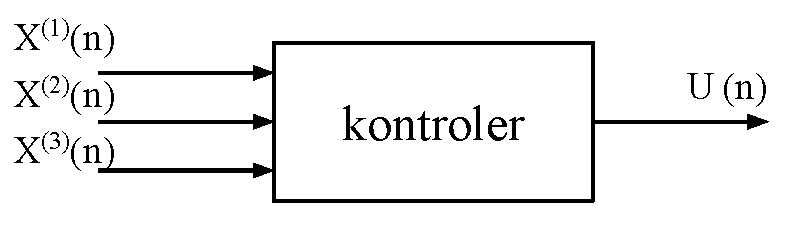
\includegraphics[width=0.5\textwidth]{images/kontroler.pdf}
    \caption{Model sterowania kontrolera}
    \label{fig:kontroler}
\end{figure}

Jak widać na rysunku \ref{fig:model} i \ref{fig:kontroler}, kontroler, do wyznaczenia ustawień sygnalizatorów, wykorzystuje wyjście sterowanego obiektu oparte o stan obiektu sterowanego.

\vspace{1.5cm}
\textbf{Parametry algorytmu}

Działanie kontrolera można konfigurować przy użyciu trzech parametrów:
\vspace{0.5cm}

\begin{math} p \in <0, 1> \end{math} \textrm{ -- wpływ przewidywanego przepływu pojazdów na sterowanie}

\begin{math} q \in <0, 1> \end{math} \textrm{ -- wpływ aktualnego przepływu pojazdów na sterowanie}

\begin{math} r \in <0, 1> \end{math} \textrm{ -- wpływ aktualnych wielkości kolejek na sterowanie}

\begin{math} p + q + r = 1 \end{math}

\begin{math} t \in \mathbb{N} \textrm{ } t > 0 \end{math} \textrm{ -- długość cyklu świetlnego}

\vspace{1.5cm}
\textbf{Stałe algorytmu}

Stałe opisują niekonfigurowalne elementy kontrolowanego zespołu skrzyżowań.
\vspace{0.5cm}

\begin{math} s \in \mathbb{N} \end{math} \textrm{ -- liczba sygnalizatorów w kontrolowanym obszarze}

\begin{math} m \in \mathbb{N} \end{math} \textrm{ -- maksymalny możliwy do zmierzenia przepływ pojazdów [liczba pojazdów/godzina]}

\begin{equation}
	\begin{array}{c}
		K_{i} = \left[ k_{i, j} \right]_{j \in <0,s>}\\
		k_{i, j} \in \mathbb{N}
	\end{array}
\end{equation}

\begin{math} k_{i, j} \end{math} \textrm{ -- maksymalna możliwa wielkość kolejki przed j-tym sygnalizatorem w i-tym obszarze [liczba pojazdów]}

\vspace{1.5cm}
\textbf{Wyjście obiektu sterowanego}

Stan sterowanego obszaru odwzorowany jest w wyjściu obiektu i opisany jest trzema zmiennymi, do sterowania wykorzystywane są wyjścia wszyskich obszarów sterowanych w postaci pojedynczego stanu systemu:
\vspace{0.5cm}

\begin{equation}
	\begin{array}{c}
		Y (n) = \left[ Y_{i} (n) \right]_{i \in <1,o>}
	\end{array}
\end{equation}

\begin{math} o \end{math} \textrm{ -- liczba obszarów sterowania}

\begin{equation}
	Y_{i} (n) = \left[
	\begin{array}{c}
		y_{i, j, 1} (n)\\
		y_{i, j, 2} (n)\\
		y_{i, j, 3} (n)\\
	\end{array}
	\right]_{j \in <1,s>}
\end{equation}

\begin{math} s \end{math} \textrm{ -- liczba sygnalizatorów w i-tym obszarze sterowania}

\begin{math} y_{i, j, 1} (n) \end{math} \textrm{ -- przepływ na dojeździe do j-tego sygnalizatora w i-tym obszarze [pojazdy/godzina]}

\begin{math} y_{i, j, 2} (n) \end{math} \textrm{ -- kolejka przed j-tym sygnalizatorem w i-tym obszarze [liczba pojazdów]}

\begin{math} y_{i, j, 3} (n) \end{math} \textrm{ -- stan j-tego sygnalizatora w i-tym obszarze}

\vspace{0.5cm}
Stany sygnalizatorów przekształcone są do postaci przewidywanego przepływu pojazdów w kierunku j-tego sygnalizatora w i-tym obszarze (\begin{math} f_{i, j} \end{math}).

\vspace{1.5cm}
\textbf{Algorytm}

Proponowany jest poniższy algorytm wyznaczania optymalnych ustawień sygnalizatorów.
\begin{enumerate}
	\item wyznaczenie wszystkich, możliwych decyzji w postaci zbiorów bezkolizyjnych ustawień sygnalizatorów, takich których strumienie ruchu nie przecinają się,
	\item wyliczenie wag sygnalizatorów, użytych później do wyznaczenia oceny decyzji, jak pokazano we wzorze \ref{eq:wagi}, im wyższa wartość wagi tym wyższy priorytet zezwolenia na ruch przez ten sygnalizator,
	\item wyliczenie funkcji oceny (\ref{eq:wagi_suma}), dla wyznaczonych wcześniej możliwych decyzji, jako sumy wag sygnalizatorów zezwalających na ruch w ramach tej decyzji,
	\item wyznaczenie optymalnej, o najwyższej wartości funkcji oceny, decyzji (\ref{eq:arg_max_q}).
\end{enumerate}

\vspace{0.5cm}
W pierwszym kroku algorytmu wyznaczane są wszystkie możliwe decyzje w postaci zbiorów bezkolizyjnych ustawień sygnalizatorów.
Spośród tak wyznaczonych zbiorów możliwy jest późniejszy wybór takiego który będzie w danym momencie optymalny.

\vspace{0.5cm}
Drugi krok pozwala wyznaczyć wagi zezwolnia na ruch przez każdy z sygnalizatorów, zgodnie ze wzorem \ref{eq:wagi}.

\begin{equation}
\label{eq:wagi}
	w_{i} (n) = p \cdot \frac{f_{i, j}}{m} + q \cdot \frac{y_{i, j, 1} (n)}{m} + r \cdot \frac{y_{i, j, 2} (n)}{k_{i}}
\end{equation}

\begin{math} w_{i} (n) \end{math} \textrm{ -- waga i-tego sygnalizatora w chwili n}

\vspace{0.5cm}
W następnym kroku, wyliczone wagi są sumowane (\ref{eq:wagi_suma}) aby wyznaczyć wartość funkcji oceny dla każdej, z przygotowanych w pierwszym kroku, decyzji.

\begin{equation}
\label{eq:wagi_suma}
	Q (X(n), S') = \sum\limit_{i \in S'} w_{i}
\end{equation}

\begin{math} S' \end{math} \textrm{ -- decyzja dla której wyznaczana jest wartość funkcji oceny}

\vspace{0.5cm}
Na końcu wybierana jest optymalna, o najwyższej funkcji oceny, decyzja (\ref{eq:arg_max_q}).

\begin{equation}
\label{eq:arg_max_q}
	S^{*} = arg\:max\:Q (X(n), S')
\end{equation}

\begin{math} S^{*} \end{math} \textrm{ -- decyzja optymalna}

\section{Uwzględnienie ograniczeń cyklów świetlnych}
Ograniczenie sekwencji faz cyklu świetlnego nie jest uwzględniane w działaniu powyżej zdefiniowanego algorytmum, podejmuje on jedynie decyzję o wydaniu zgody na ruch.

\begin{equation}
	S^{*} \to U(n)
\end{equation}

Za przestrzeganie tego jak i innych, czasowych, ograniczeń odpowiada dodatkowy komponent który przekazuje do obiektu sterowanego ostateczną decyzję. Zmiana sygnału powoduje utworzenie sekwencji sygnałów które nastąpią w kolejnych chwilach czasu. Uruchomienie sygnału zielonego jest opóźnione przez uwzględnienie czasów międzyzielonych. Również ograniczenia długości sygnałów żółtego i czerwono-żółtego są aplikowane na tym etapie. Wspomniany komponent odpowiada też za wymuszenie uruchomienia sygnału czerwonego, jak i zielonego, przynajmniej raz na cykl świetlny.

\section{Metody oceny skuteczności algorytmu}
Do oceny skuteczności algorytmu wykorzystać można określone na podstawie pracy Piotra Kawalca i Sylwii Sobieszuk-Durki \cite{kawalec+sobieszuk-durka} metody oceny. Są to:
\begin{itemize}
	\item średnie czasy przejazdu pojazdów na wybranych trasach
	\item średnialiczba zatrzymań pojazdów
	\item średnia prędkość pojazdów
\end{itemize}

Określone w ten sposób metody oceny można wykorzystać do porównania algorytmu z przypadkiem braku sterowania czy sterowaniem przy użyciu stałoczasowego, niezsynchronizowanego, programu sygnalizacji. Ocena wyników badań znajduje się w rozdziale \ref{chap:ocena}.